\chapter{Energy Estimators}
\label{chap:MoreStuff}

\chapterquote{There, sir! that is the perfection of vessels!}
{Jules Verne, 1828--1905}

\section{Calibration}

\subsection{Calibration in the particle flow paradigm}

%Say why calibration is important and how it fits into particle flow

In any experiment, calibration is essential for ensuring reliability in measured quantities and the linear collider will be no exception to this.  At the linear collider there will be several measured quantities each of which will be converted into a measure of the energy deposited in a given region of the detector.  These fall into two distinct classes (i) calorimeter energy deposits and (ii) track deposits.  The focus of this section will be on the energy deposits in the calorimeter and the procedure developed to ensure that they are reliable.  

Calorimeter energy deposits are an essential building blocks for the application of the particle flow paradigm.  The separation of energy deposits from charged and neutral particles in the calorimeters is crucial to achieve the full potential of particle flow and this is only possible with accurate energy estimators for those energy deposits.  A robust calibration scheme has been developed and will be discussed in the following chapter. 

The other crucial energy deposit used in particle flow claorimetry are track energy deposits.  These are also crucial to physics performance, however, in the particle flow paradigm these energy depsoits are topologically related to the energy of the reconstructed particle.  A spatial helix fit is applied to the track energy deposits which when combined with knowledge of the magnetic filed yeilds the momentum of the particle producing the track.  Therefore, there is no direct relationship between the energy deposited by the monte-carlo particle in the active medium and the energy of the reconstructed energy.  Therefore, precise calibration of the energy deposited by a charged particle track is less crucial than for calorimeter energy deposits.  For this reason the focus of this chapter is on the calibration of calorimeter energy deposits. 

Calibration of the linear collider simulation extends beyond the raw calorimeter hits and into the particle flow algorithm itself.  The fine calorimeter granularity required for particle flow calorimetry yeilds excellent physical separation of hadronic and electormangetic showers.  Thanks to sophisticatd particle identification occuring within PandoraPFA it is possible to distinguish hadronic and electormangetic showers, which allows for distinct treatments of the hadronic and electromangetic energy estimators.  This distinction can be used to produce a response from the calorimeter that is compensating despite the intrinsic response being non-compensating.  A compensating calorimeter would give significant improvmetns to the energy resolution for the detector.

Two treatments designed to achieve a compensating response from the calorimeters are discussed.  The both involve rescaling the energies, the first rescaling is applied using a series of fixed energy independant constants, while the second uses the energy density of the calorimeter hits in the shower to determine the energy rescaling factor.

\subsection{Calibration and detector optimisation}

% Say why calibration important for detector optimisation 

Optimising the detector at a future linear collider will be crucial to exploit the full physiscs potential available to it.  An extensive optimisation of the calorimeters was performed the results of which can be found in chapter ....  However, this study would not have been possible without the development of a robust and well motivated calibration procedure.  This procedure had to be robust so that it could be applied to multiple detector concepts and well motivated so that true physics potential of each detector was realised.

\subsection{Calibration Goals}

The three cornerstone goals of the calibration procedure are as follows

\begin{enumerate}
\item MIP scale setting.  This step sets the response of the detector to minimally ionising particles (MIPs).  This is a useful scale to set for comparison to physically well motivated energy comparisons and thus is used by several different algorithms in a typical reconstruction chain. 
\item Digitisation of calorimeter hits.  At this stage the energy deposited in the active layers of a calorimeter, e.g. Si layers, are used to estimate the energy deposited in the absorber layers of the calorimeter.  
\item Electromagnetic and hadronic scale setting.  In this step the energy deposits from electromagnetic and hadronic showers are, having been distinguished by the pattern recongition software, are independantly rescaled to account for the invisble energy component of hadronic showers.  
\end{enumerate}

Each of these aspects needs separately addressing for each new detector model considered.  The ordering of each of these calibration steps also had to be taken into consideration as it is possible to get interference between the different stages if applied in the wrong order.  For example setting the MIP scale in PandoraPFA requires post digitsation calorimeter hit and so must be done post digitisation of the calorimeter hits to be accurate.

\subsection{Digitisation}
% How digitsation is applied
The goal of the digitisation step of the calibration procedure is to ensure an accurate estimation of the energy deposited in the absorber layers of the calorimeter based on the energy deposits in the active layers.  The energy deposited in a given calorimeter cell, containing an active and absorber layer pair, is assumed to be equal to a constant, hereby known as a digitsation constant, multipled by the energy measured within the active layer.  This approximation holds true given a sufficiently high spatial sampling of the shower that variations in the longitudinal energy deposition profile across the cells are negligible.  

The digitisation constants depend upon several aspects of the detector including the material properties of the active and absorber layers, the magnetic field strength in the region of the subdetector and energy losses occuring within the gaps between the active and absorber layers.  Some dead material between the active and aborber layer is simulated in the detector to give the effect of the instrumented read out technology that would exist in a completed detector.  The empirical calculation of these constants for each subdetector is discussed below. 

% How the empirical calculation works
The procedure for determining the digitisation constants is as follows, fixed energy single particle events are simulated that are fully contained within the detector.  As the calibration procedure is iterative the first step applies a trial calibration that may contain miscalibration.  The energy of the calorimeter hits are summed on an event by event basis.  This distribution should, for an ideal calorimeter, be Gaussian as described in section BLAH, therefore, a Gaussian fit is applied to this distribtuion and the mean extracted.  For the case of perfect calibration the mean of this fit would be equal to the MC energy of the simulated single particle events, therefore, it is assumed that any deviation from the MC energy is due to miscalibration.  To correct for this offset the digitsation constant from the trial calibration is rescaled by the ratio of the MC energy to mean of the fitted distribution.

\begin{equation}
\alpha_{Digi0} \rightarrow \alpha_{Digi} = \alpha_{Digi0} \times \frac{E_{MC}}{E_{Gauss}}
\end{equation}

% Each detector needs its own constants to be calibrated separately 
Due to the different physcial structure and positioning of the subdetectors in a full detector, each subdetector system will require a distinct digitisation constant that will require calibrating.  The calibration is applied independantly to each subdetector system to ensure that the assumption that the distribution of calorimeter hits in a given subdetector should, for perfect calibration, be centred on the MC energy of the single particle events in use.  This assumption also replies upon the fact that leakage out of the back of the subdetector is not a dominant effect.  Details on how this is accounted for are given below.

\subsubsection{ECal Digitisation}

% Choice of photon for ECal and event selection
The first subdetector system to be considered is the electromagnetic calorimeter (ECal).  The primary goal of the ECal is to record energy deposits from electromagentic showers.  Therefore, photons at a fixed energy of 10 GeV are used as the single particle sample for calibration.  Photon energy measurements in the particle flow paradigm arise from the calorimeter energy deposits, specifically those in the ECal, therefore they were an obvious choice of calibration event.  Electrons could have been used for this stage of the calibration as such events would also yeild electromagnetic showers, however, the reconstructed energy from such events would ultimately come from the track measurment.  

% Contained events 

The choice of photons helps with the issue of contained events as, due to the large number of radiation legnths typically found in the ECal, the events will be largely contained entirely within this subdetector.  This statement doesn't hold at extremely large energies, however, at 10 GeV is it sufficient to say that the photon events are contained in the ECal as figure \ref{engest:fig:energysplitphotondigi} shows.

\begin{figure}
  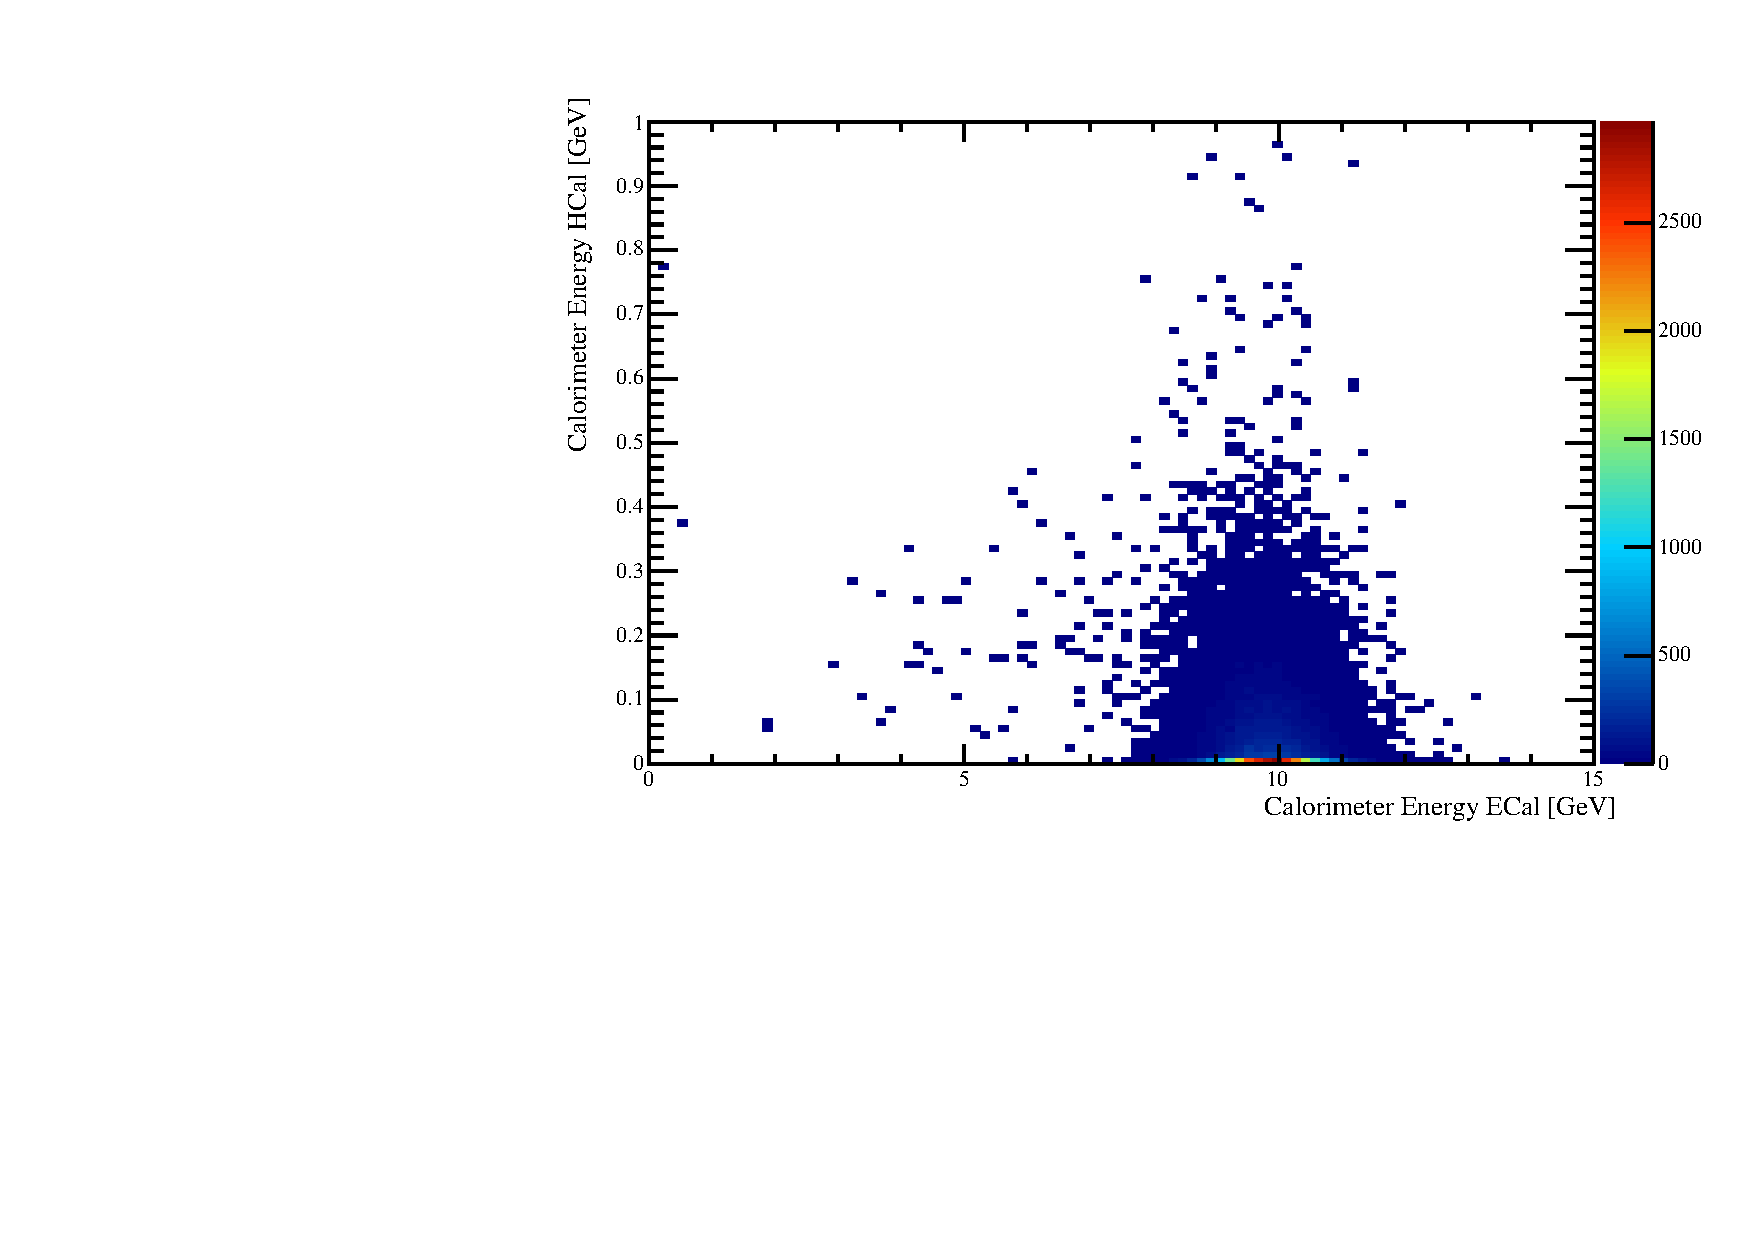
\includegraphics[width=\largefigwidth]{EnergyEstimators/Plots/Calibration/Digitsation/ECal/10GeVPhotonEnergyECalHCal.pdf}
  \caption[Sum of calorimeter hit energies in ECal and HCal for 10 GeV photons.]{Sum of calorimeter hit energies in ECal and HCal for 10 GeV photons.}
  \label{engest:fig:energysplitphotondigi}
\end{figure}

% Cuts on event selection
The photon event sample was generated with fixed energy uniformly in solid angle.  To excude events passing down the beam line a cut on the polar angle, $\theta$, of the magnitude of cos$\theta$ to be less than 0.95 was applied to the reconsturcted PFOs.  To veto photon conversion events ($\gamma \rightarrow e^{+}e^{-}$ pair creation) events from the calibration sample it was required that there be a single photon target (*explain PFO targets).  Finally, to ensure that events were contained within the ECal it was required that at least 99\% of the event energy occur within the ECal.  The effect of these preselection cuts on a typical calibration sample is shown in figure \ref{engest:fig:cutsphotondigi}.  

\begin{figure}
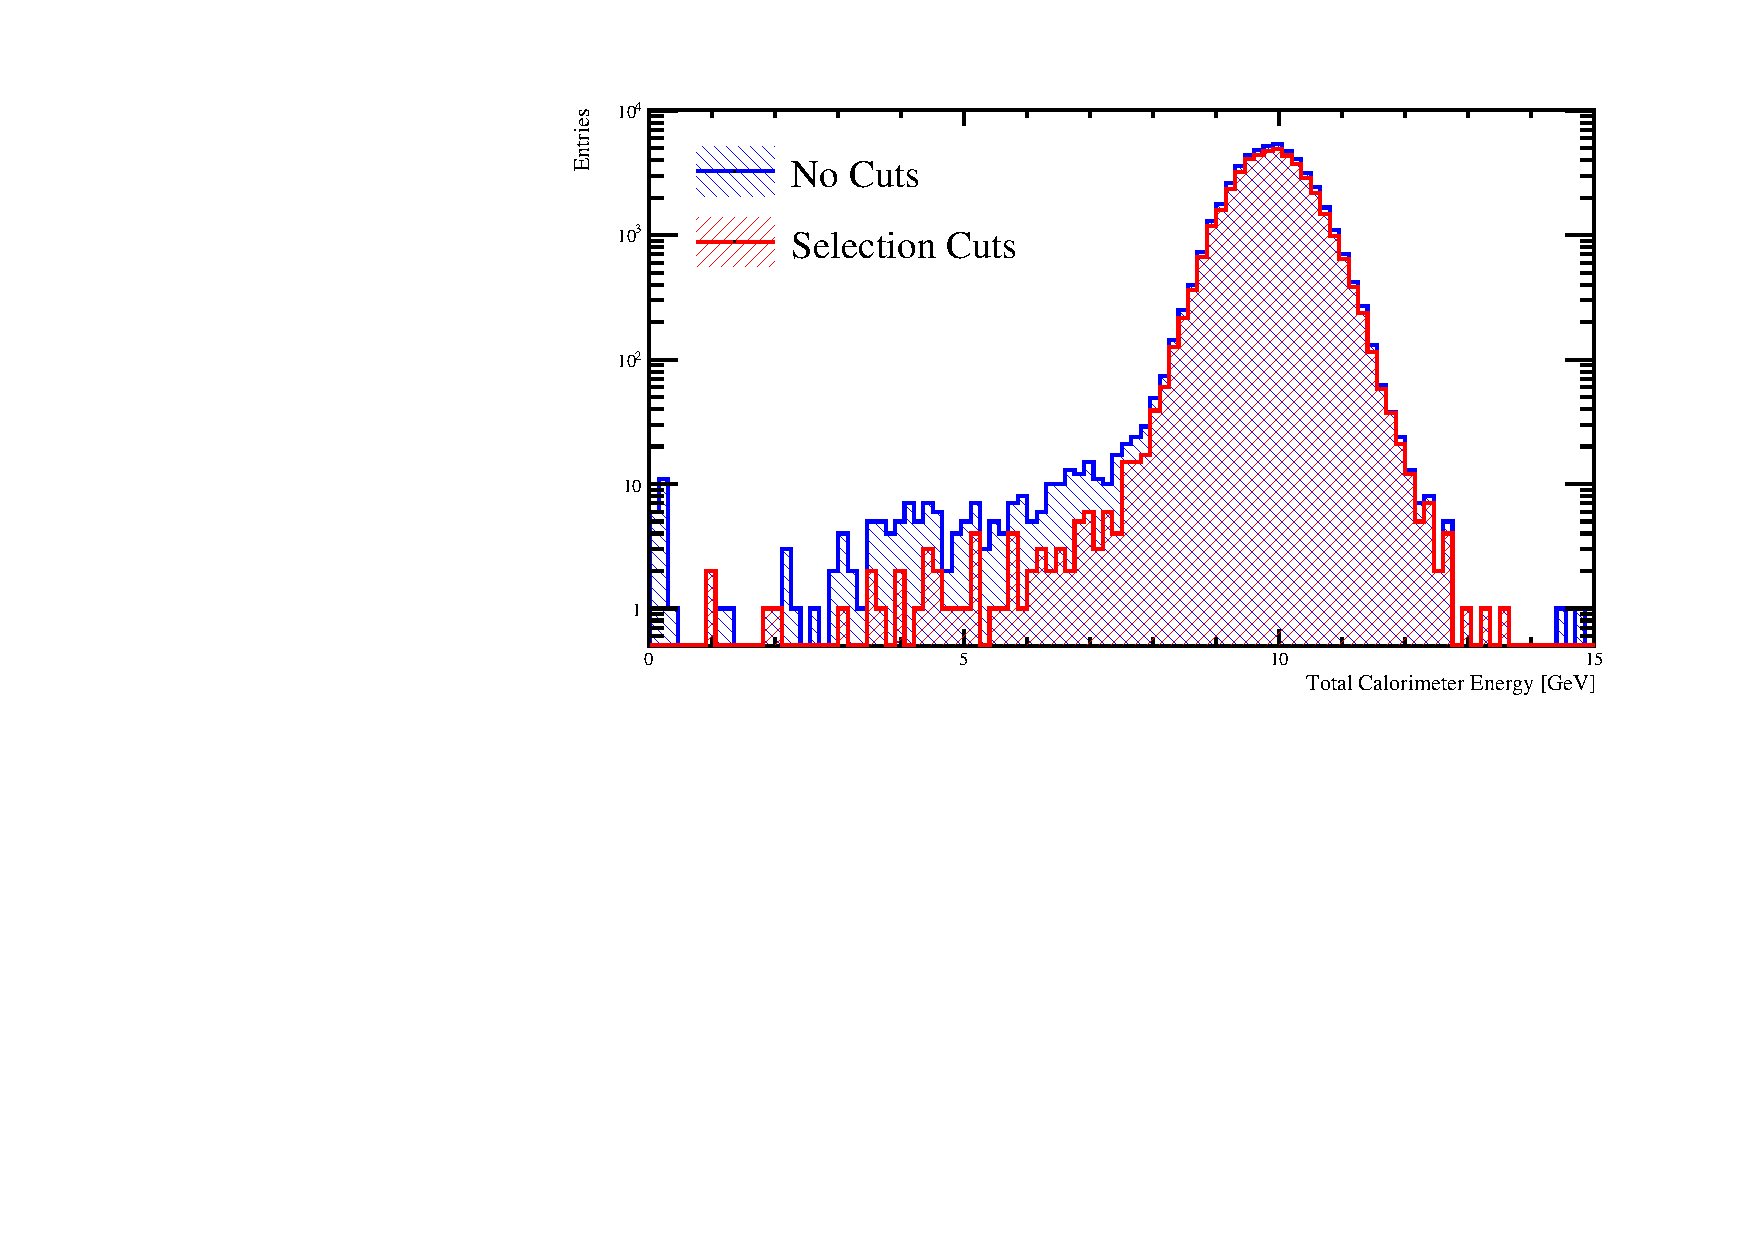
\includegraphics[width=\largefigwidth]{EnergyEstimators/Plots/Calibration/Digitsation/ECal/ECalDigiCuts.pdf}
  \caption[Sum of the raw calorimeter hit energies for a 10 GeV photon with and without the preselection cuts.]{Sum of the raw calorimeter hit energies for a 10 GeV photon with and without the preselection cuts.}
  \label{engest:fig:cutsphotondigi}
\end{figure}

% Still not perfectly Gaussian 
As figure \ref{engest:fig:cutsphotondigi} shows there are still some outlying events in the distribution.  These are most likely due to events that encounter gaps between detector modeules in the simulation.  This means that they encounter much less material in the simulation than expected and could potentailly shower much deeper into the calorimeters than expected.  An example event suffering from the effect of detector gaps is shown in figure BLAH.



\subsection{MIP Scale Setting}


\subsection{Electromagnetic and hadronic scale setting}




\begin{figure}
  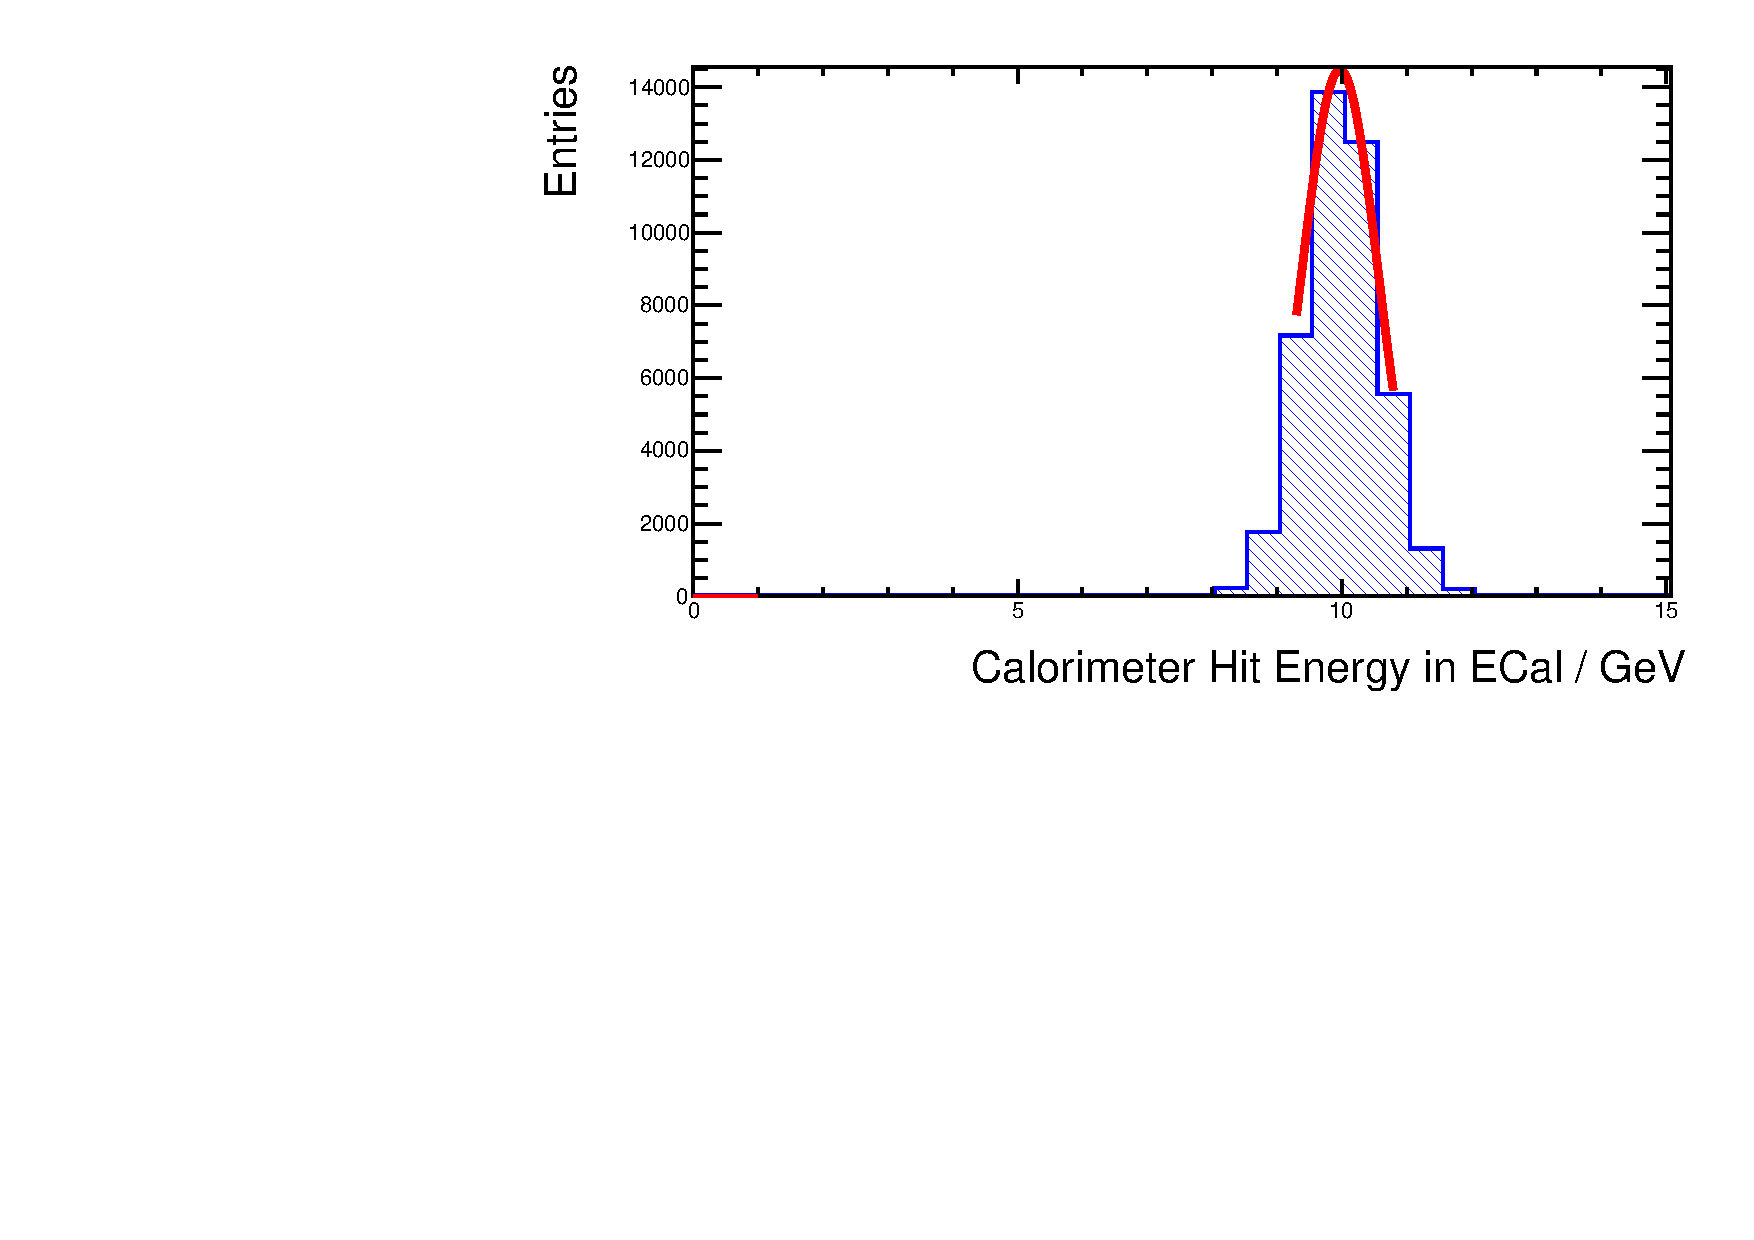
\includegraphics[width=\largefigwidth]{EnergyEstimators/Plots/Calibration/ECalDigitsation.pdf}
  \caption[Sum of the raw calorimeter hit energies for a 10 GeV photon.]{Sum of the raw calorimeter hit energies for a 10 GeV photon.}
  \label{engest:fig:ecaldigi}
\end{figure}




\subsection{Compensating Calorimeter}

By accurately determining these rescaling values it is possible to apply an energy correction to compensate for the invisible energy component of hadronic showers.  This invisible componenet arises from mechanisms such as low energy neutron release and nuclear binding energy losses amongst other such processes.  Discussion of this procedure and how to calibrate such a process is the main focus of this section.  


\begin{figure}
  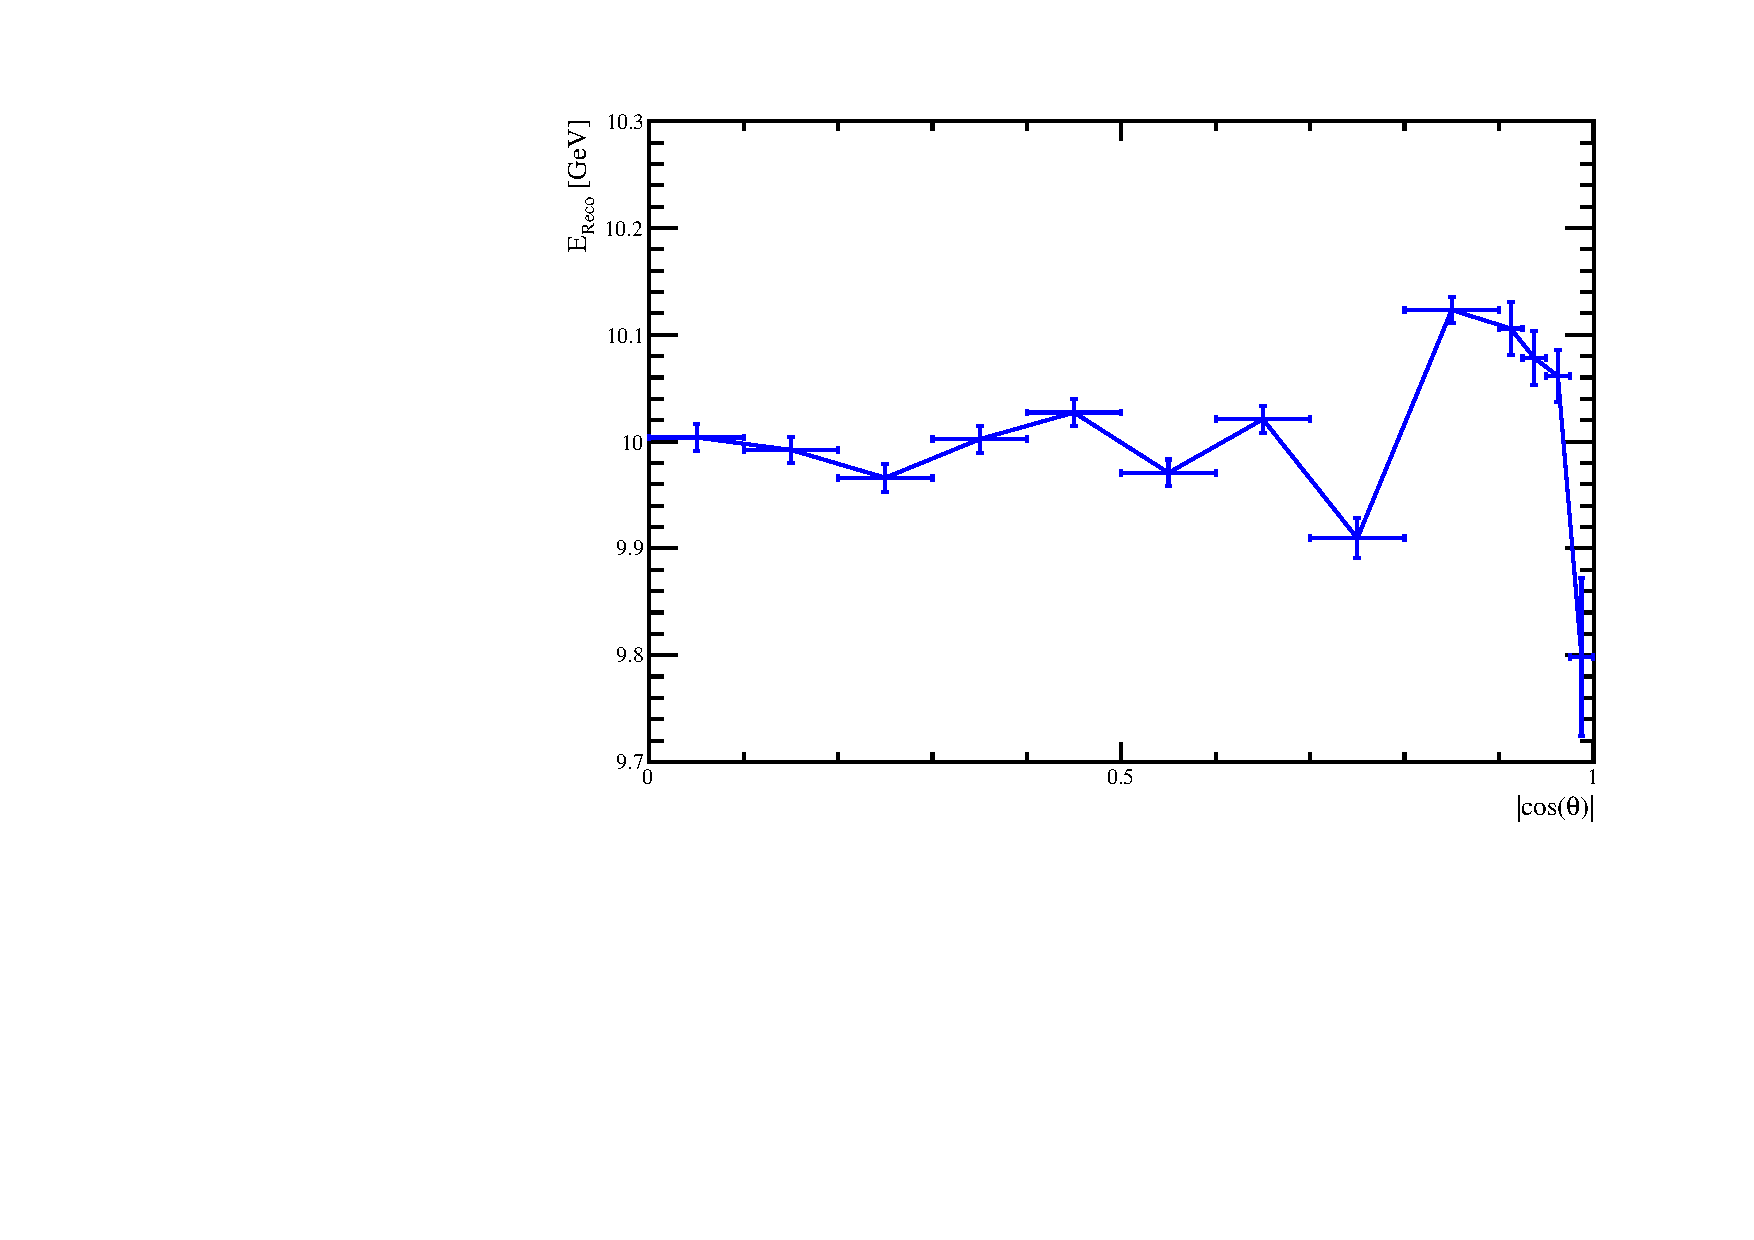
\includegraphics[width=\largefigwidth]{EnergyEstimators/Plots/Calibration/Validation/AngularDistributionPhotonPlot.pdf}
  \caption[Mean reconstructed photon energy as a function of the polar angle of the photon.]{Mean reconstructed photon energy as a function of the polar angle of the photon.}
  \label{engest:fig:photonangle}
\end{figure}

\begin{figure}
  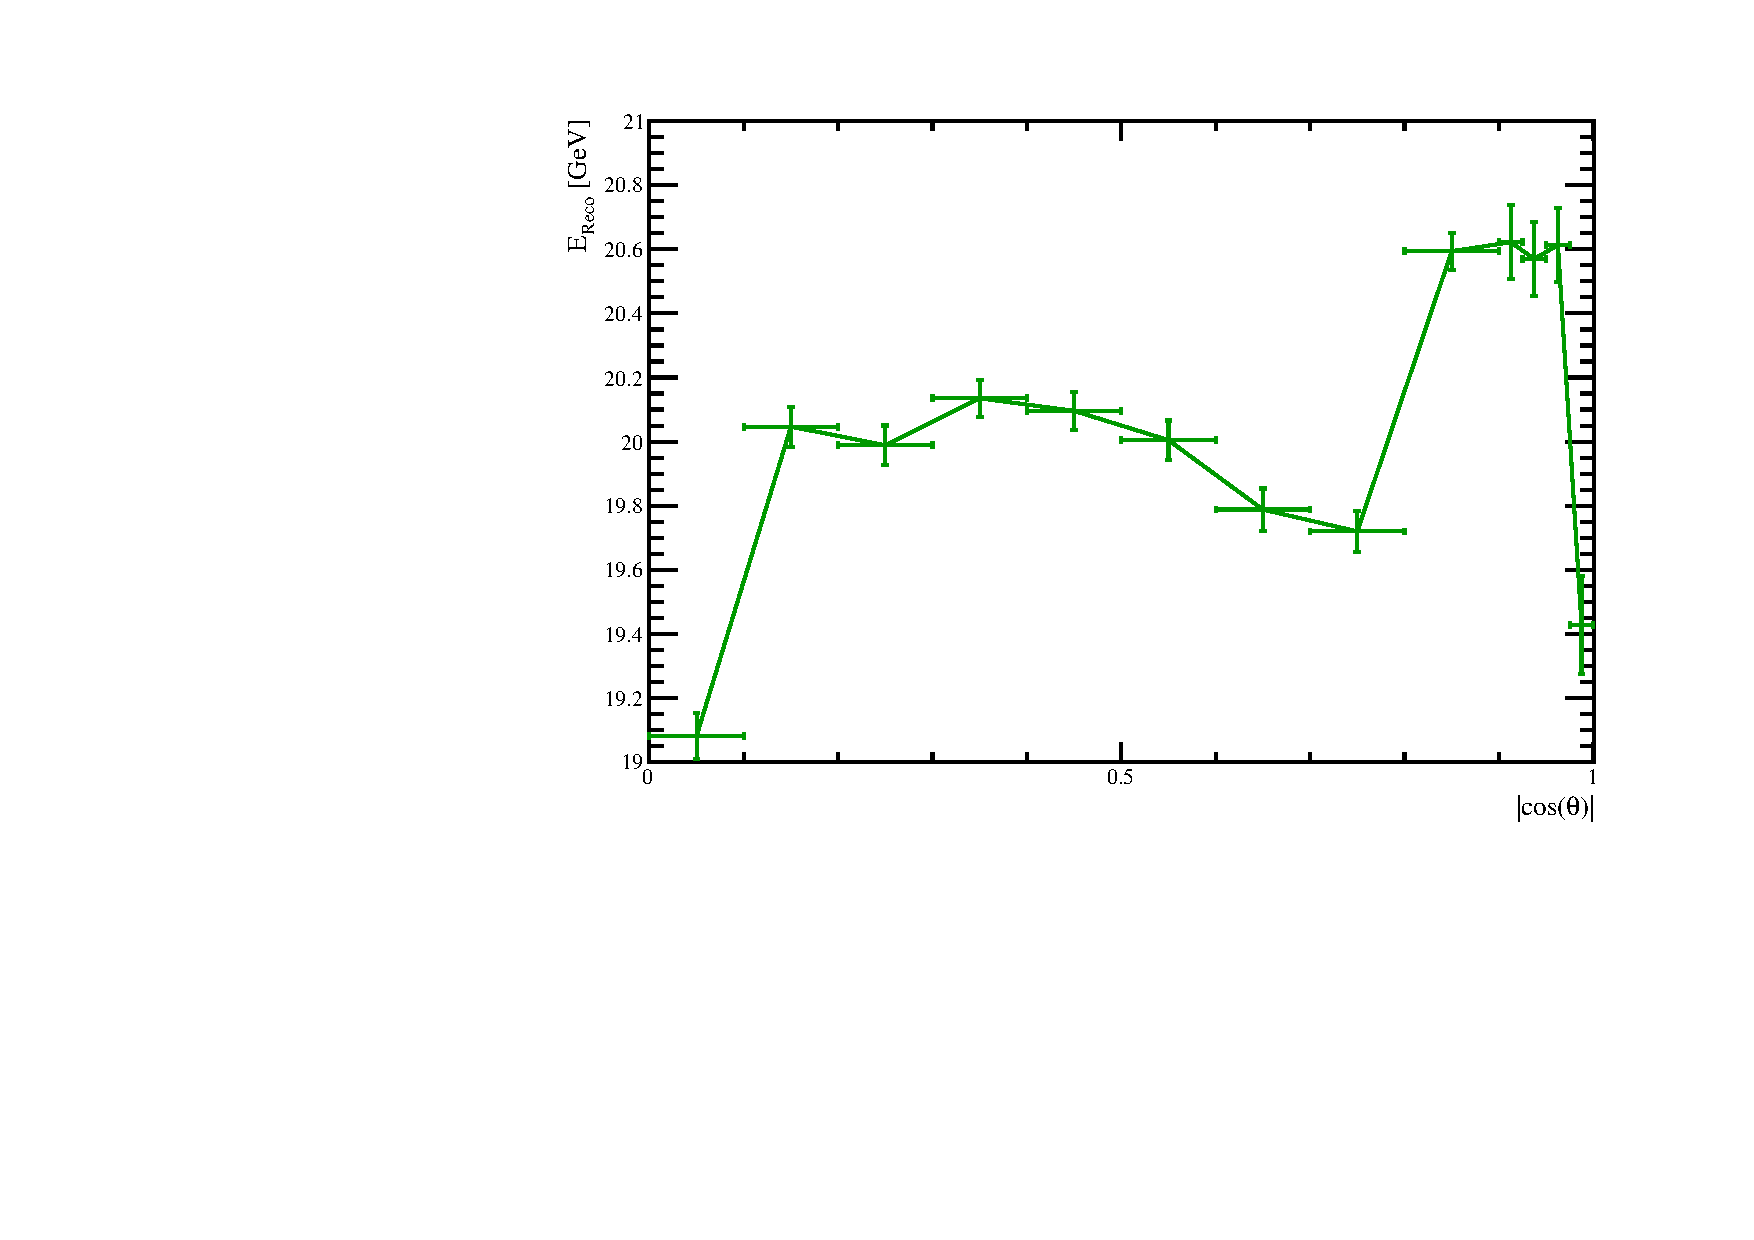
\includegraphics[width=\largefigwidth]{EnergyEstimators/Plots/Calibration/Validation/AngularDistributionKaon0LPlot.pdf}  \caption[Mean reconstructed kaon0L energy as a function of the polar angle of the kaon0L.]{Mean reconstructed kaon0L energy as a function of the polar angle of the kaon0L.}
    \label{engest:fig:photonangle}
    \end{figure}


\iffalse
Validation 
/Users/stevengreen/Thesis/EnergyEstimators/Plots/Calibration/Validation
207:Validation stevengreen
AngularDistributionKaon0LPlot.pdf AngularDistributionPhotonPlot.pdf

SoftComp
/Users/stevengreen/Thesis/EnergyEstimators/Plots/SoftComp/DrawWeights.C /Users/stevengreen/Thesis/EnergyEstimators/Plots/SoftComp/MakePlots.C /Users/stevengreen/Thesis/EnergyEstimators/Plots/SoftComp/PfoEnergyKaon0L.C /Users/stevengreen/Thesis/EnergyEstimators/Plots/SoftComp/PFOEnergySoftComp.pdf /Users/stevengreen/Thesis/EnergyEstimators/Plots/SoftComp/Weights.C 

Calibration
/Users/stevengreen/Thesis/EnergyEstimators/Plots/Calibration/Calorimeter_Hit_Energies_ECal_Digitisation.C /Users/stevengreen/Thesis/EnergyEstimators/Plots/Calibration/Calorimeter_Hit_Energies_HCal_Barrel_Digitisation.C /Users/stevengreen/Thesis/EnergyEstimators/Plots/Calibration/Calorimeter_Hit_Energies_HCal_EndCap_Digitisation.C /Users/stevengreen/Thesis/EnergyEstimators/Plots/Calibration/Direction_Corrected_SimCalorimeterHit_Energy_Distribution_ECal_10_GeV_Muons.C /Users/stevengreen/Thesis/EnergyEstimators/Plots/Calibration/Direction_Corrected_SimCalorimeterHit_Energy_Distribution_HCal_10_GeV_Muons.C /Users/stevengreen/Thesis/EnergyEstimators/Plots/Calibration/Direction_Correction_Distribution_HCal_20_GeV_KaonL.C /Users/stevengreen/Thesis/EnergyEstimators/Plots/Calibration/ECalDigitsation.pdf /Users/stevengreen/Thesis/EnergyEstimators/Plots/Calibration/EMPandora.pdf /Users/stevengreen/Thesis/EnergyEstimators/Plots/Calibration/GeVToMIP_Calibration_10_GeV_Muons_ECal.C /Users/stevengreen/Thesis/EnergyEstimators/Plots/Calibration/GeVToMIP_Calibration_10_GeV_Muons_HCal.C /Users/stevengreen/Thesis/EnergyEstimators/Plots/Calibration/GeVToMIP_Calibration_10_GeV_Muons_Muon_Chamber.C /Users/stevengreen/Thesis/EnergyEstimators/Plots/Calibration/HadPandora.pdf /Users/stevengreen/Thesis/EnergyEstimators/Plots/Calibration/HCalDigi.pdf /Users/stevengreen/Thesis/EnergyEstimators/Plots/Calibration/MIPResponseECalDigi.pdf /Users/stevengreen/Thesis/EnergyEstimators/Plots/Calibration/MIPScalePandora.pdf /Users/stevengreen/Thesis/EnergyEstimators/Plots/Calibration/PandoraPFA_Calibration_Electromagnetic_Energy_Scale_10_GeV_Photons.C /Users/stevengreen/Thesis/EnergyEstimators/Plots/Calibration/PandoraPFA_Calibration_Hadronic_Energy_Scale_Chi_Sqaured_Method_20_GeV_KaonL.C 
\fi


